\nonumsec{Introduction}	

%--------------------------------------------------------------------------------------------------
\begin{frame}[t]
    \frametitle{Motivation: Low stakes}
    My go to exercise is running, \textbf{but...}\pause
    \begin{figure}
        \centering
        \begin{tikzpicture}[font={\scriptsize}]
            \node[align=center] (text_1) at (0,4) {I think my running shoes \\
                are getting \emph{worn}};
            \node (img_in) at (0, 1.25) {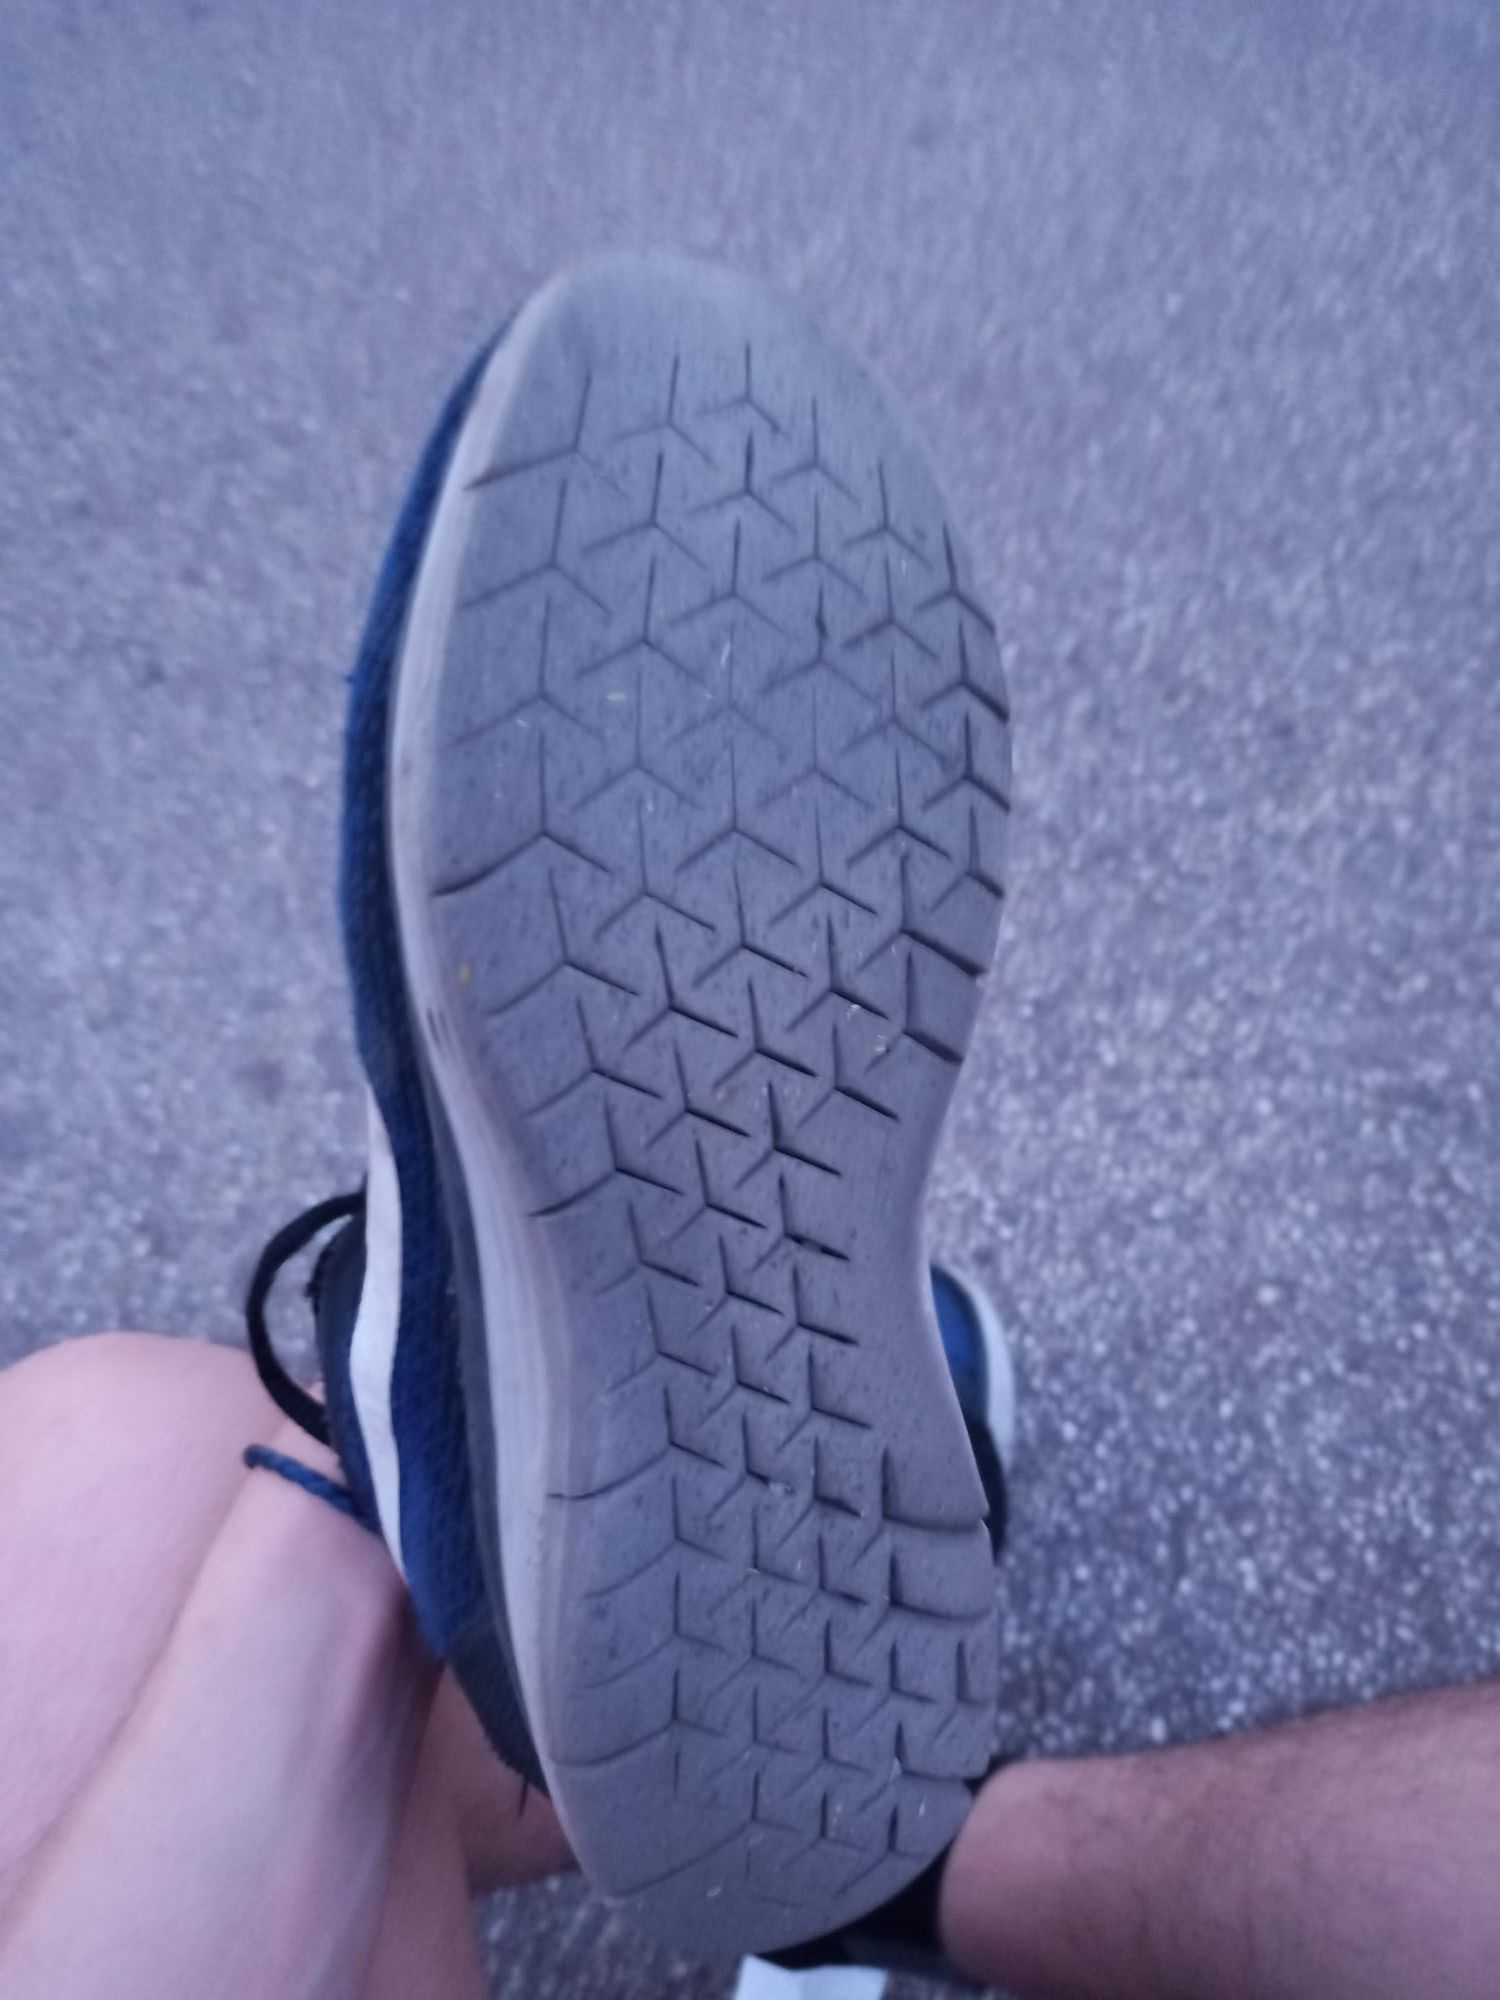
\includegraphics[scale=0.06]
                {fig/intro/motivation/lo_stakes/tired_boss}};
            \pause
            \node[align=center] (text_2) at (3.5, 4) {I want a replacement, \\ 
                 \emph{but} I know about\\machines, not shoes!};
            \pause
            \node[align=center] (text_5) at (3.5, -0.75) {\emph{still}, I know my phone can \\
                \emph{identify} my current shoes};
            \node (img_shoe_raw) at (3.5,1.45) {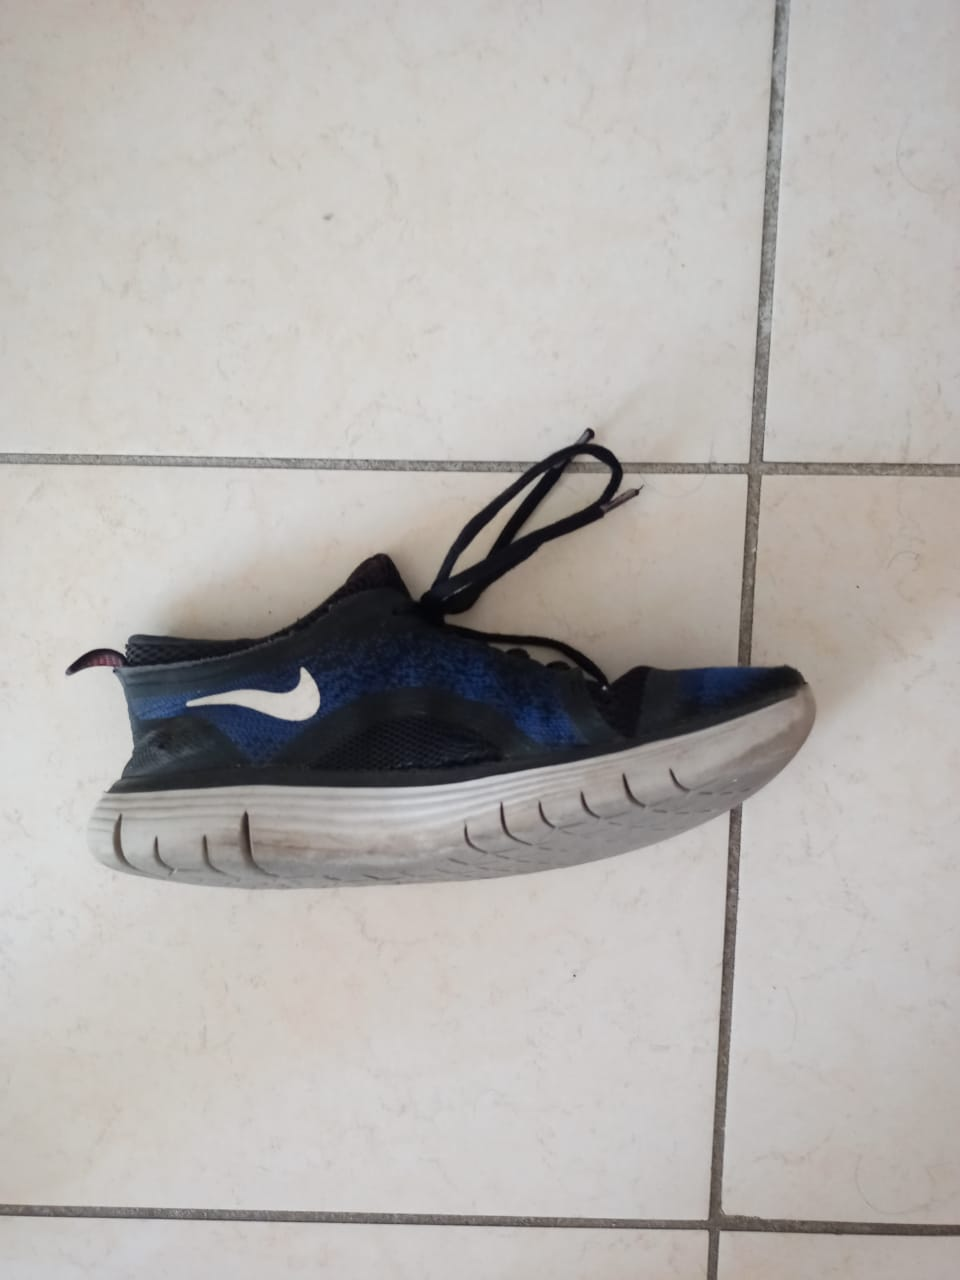
\includegraphics[scale=0.07]
                {fig/intro/motivation/lo_stakes/shoe_current}};
            \pause
            \node (img_zeros) at (3.5,1.45) 
                {
\includegraphics[scale=0.1]{fig/intro/motivation/lo_stakes/zeros_img.jpeg}};
            \node (img_idd) at (3.5,1.45) 
                {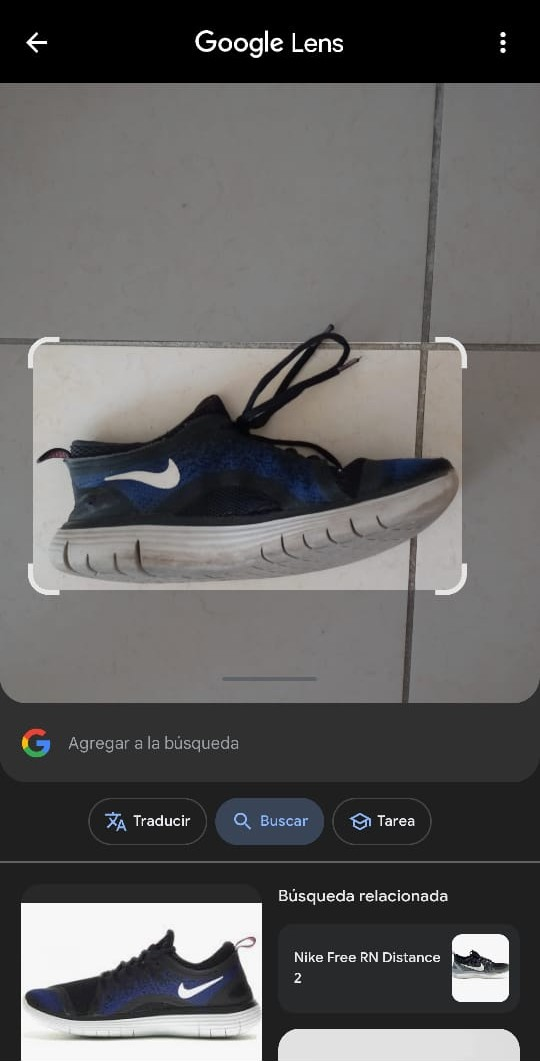
\includegraphics[scale=0.09]{fig/intro/motivation/lo_stakes/shoe_lens.jpeg}};
            \node[align=center] (text_brand_new) at (7, 3) {and obtain a new pair \\
                                                of the shoes I like};
            \node (img_brand_new) at (7, 1.75) 
            {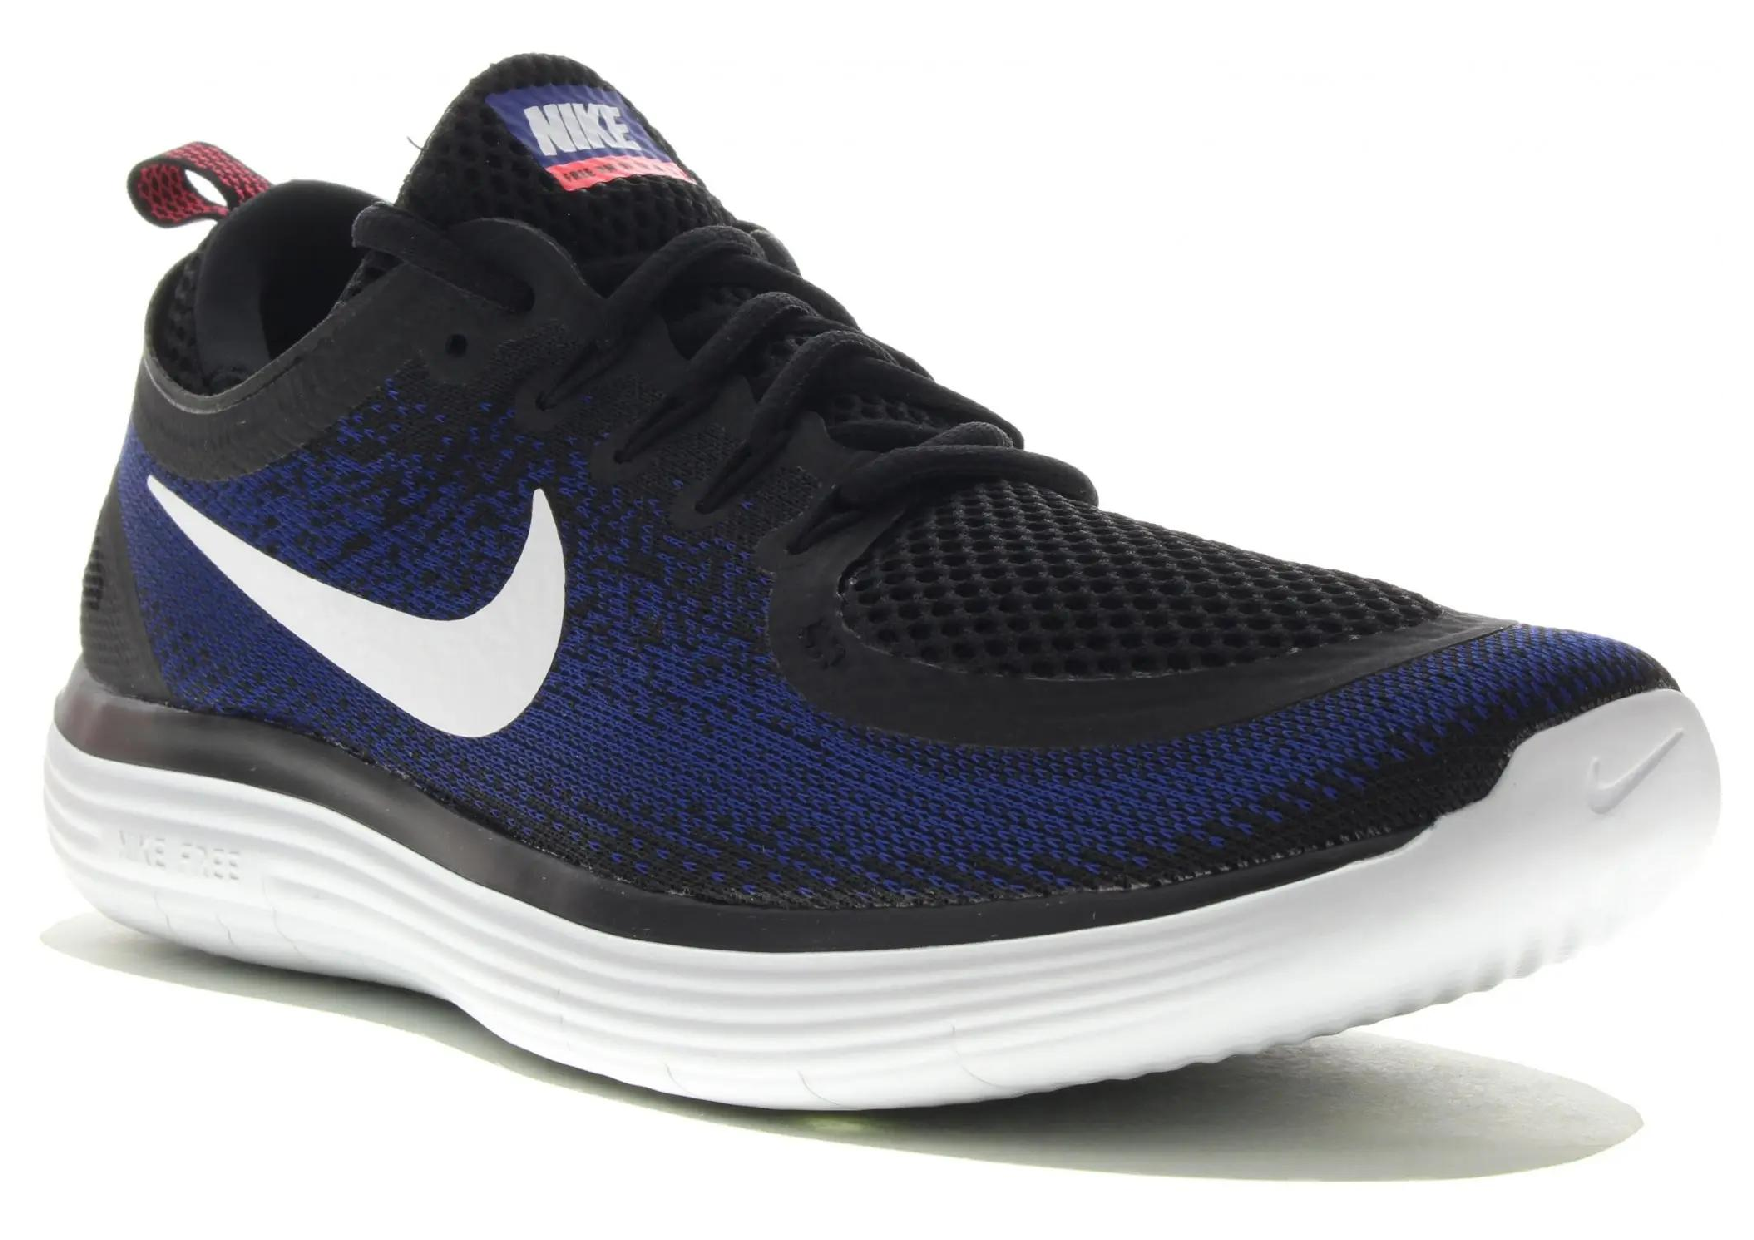
\includegraphics[scale=0.05]{fig/intro/motivation/lo_stakes/brand_new}};
            \node[align=center] at (img_brand_new.south) {The \emph{Nike Free RN Distance 2}};
        \end{tikzpicture}        
    \end{figure}
\end{frame}
 %--------------------------------------------------------------------------------------------------
\begin{frame}[t]
    \frametitle{Motivation: Raising the stakes}
    Now let's consider riskier situations:
    \pause
    \begin{figure}
        \centering
        \begin{tikzpicture}[font={\scriptsize}]
            \node (cancer) at (current page.north west) 
                {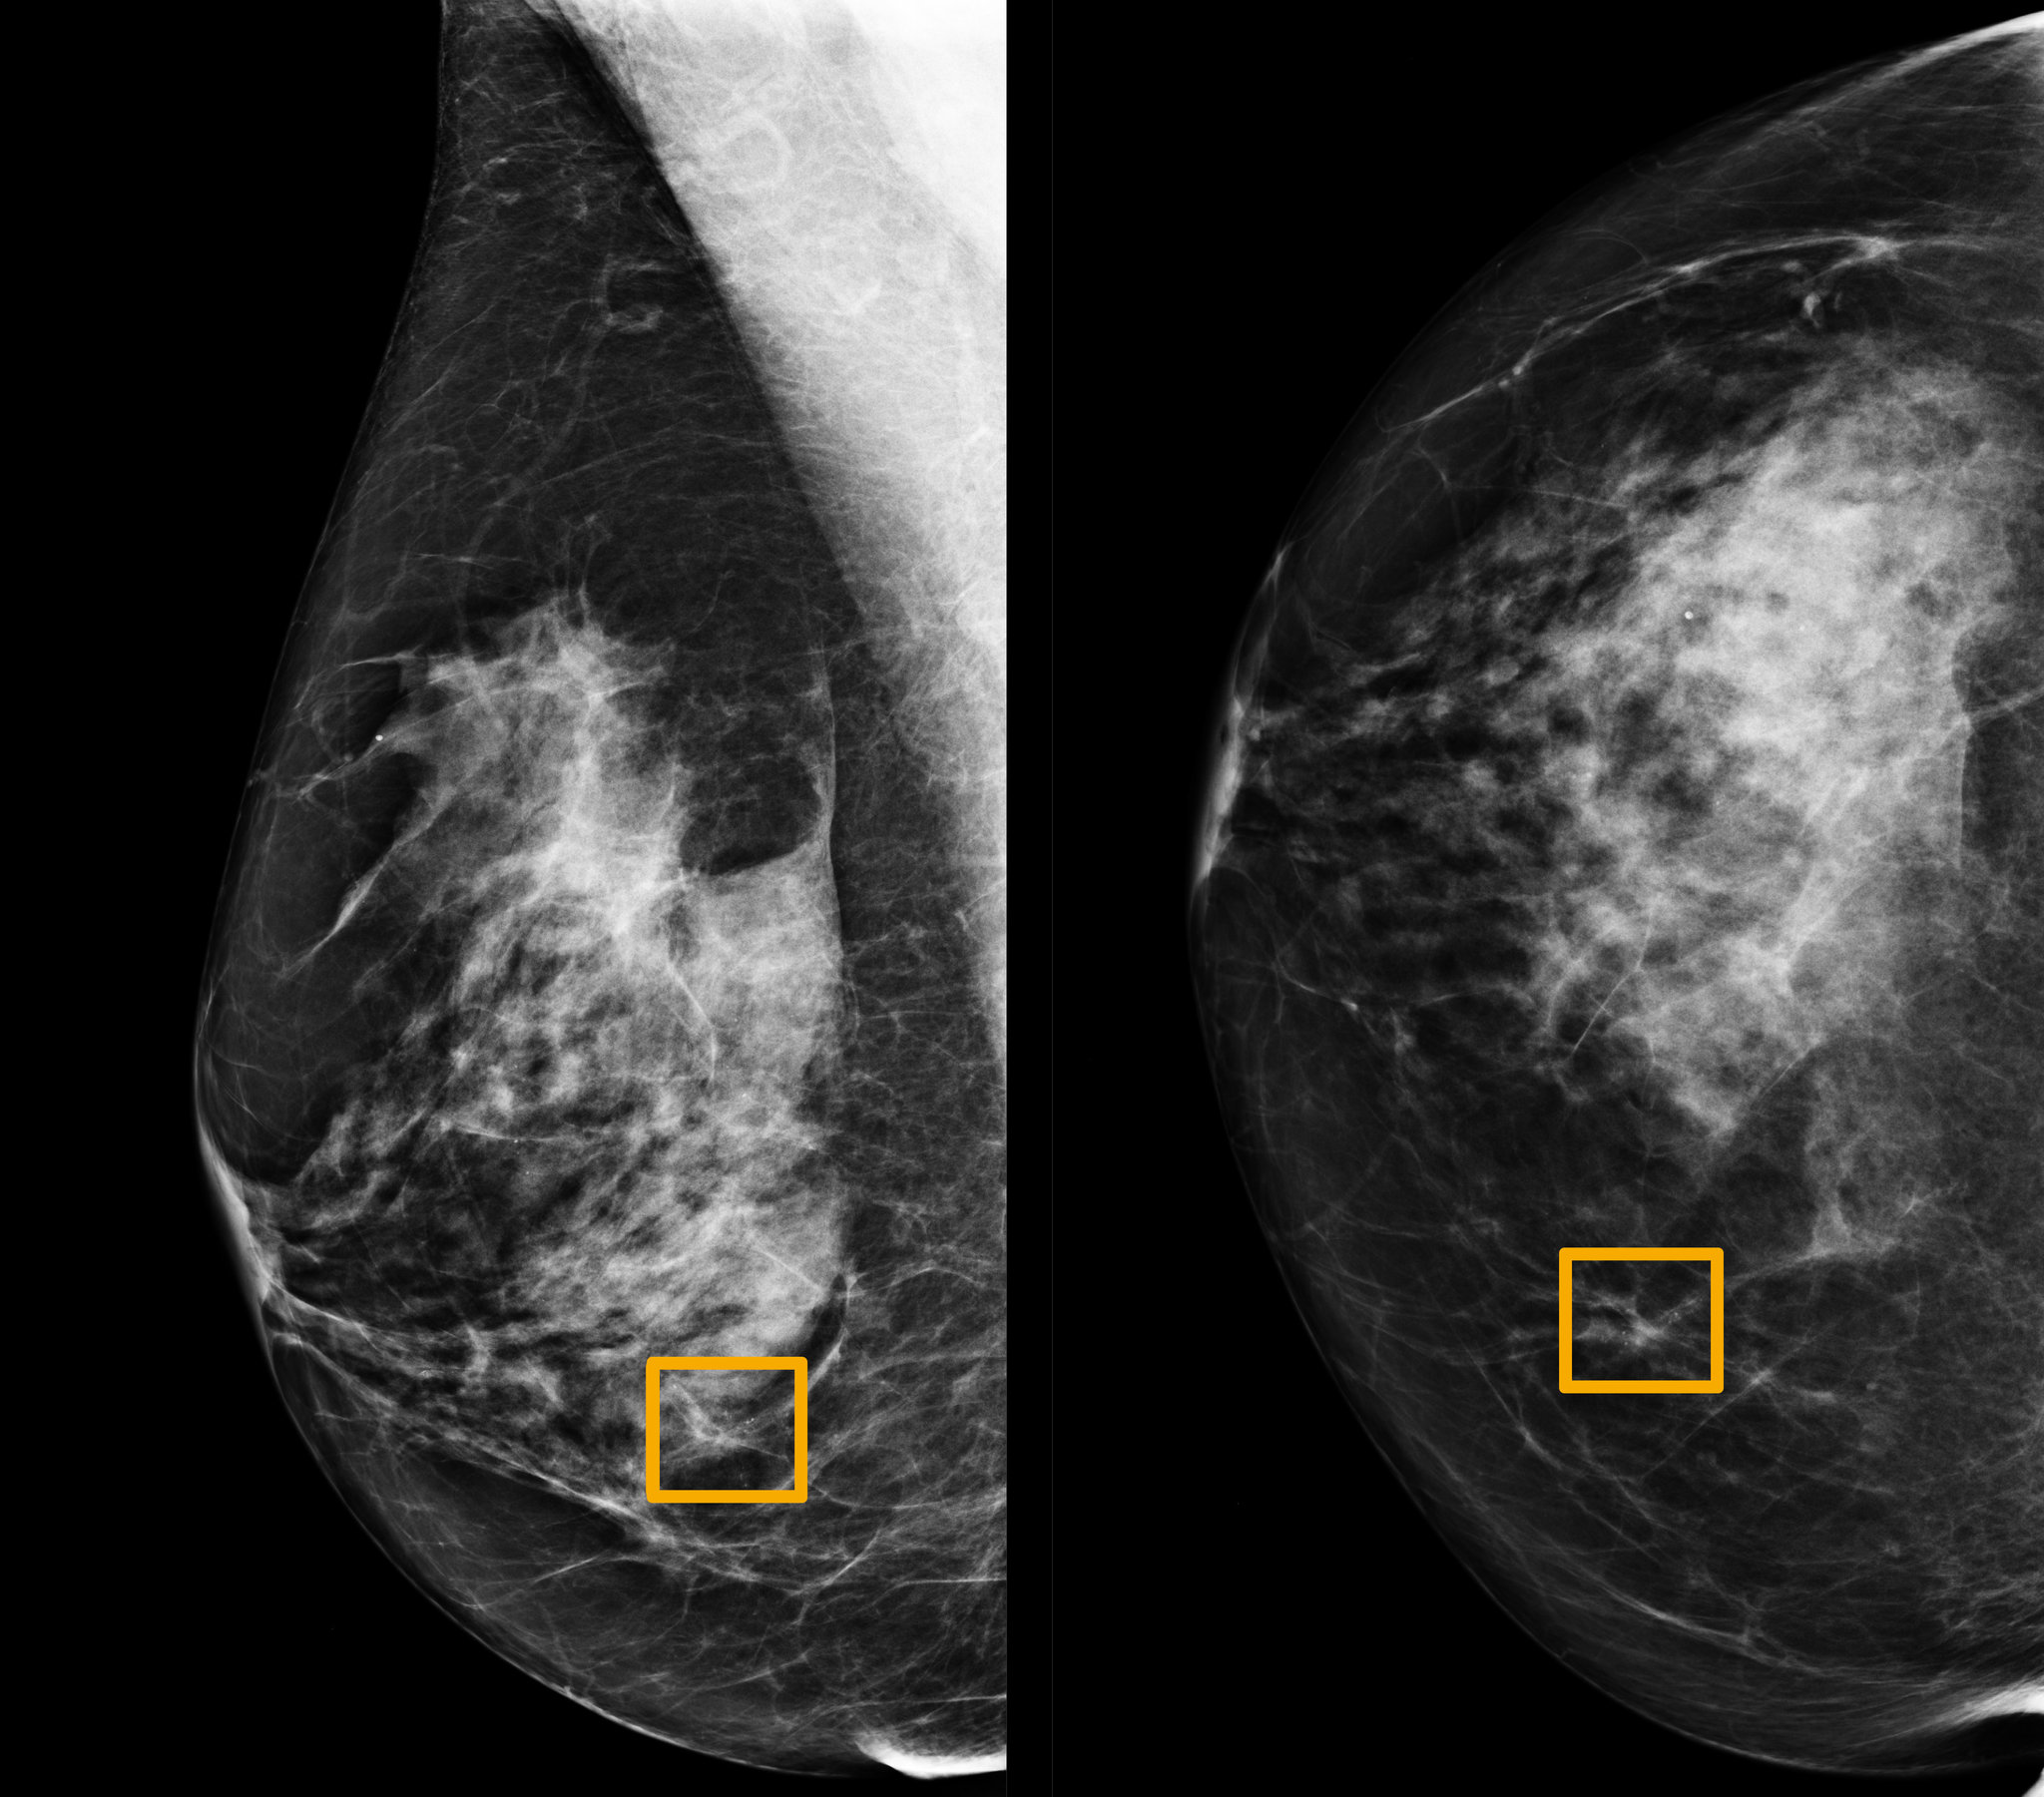
\includegraphics[scale=.07]{fig/intro/motivation/hi_stakes/breast_xray.jpg}};
            \pause
            \node (reid) at (cancer.south) {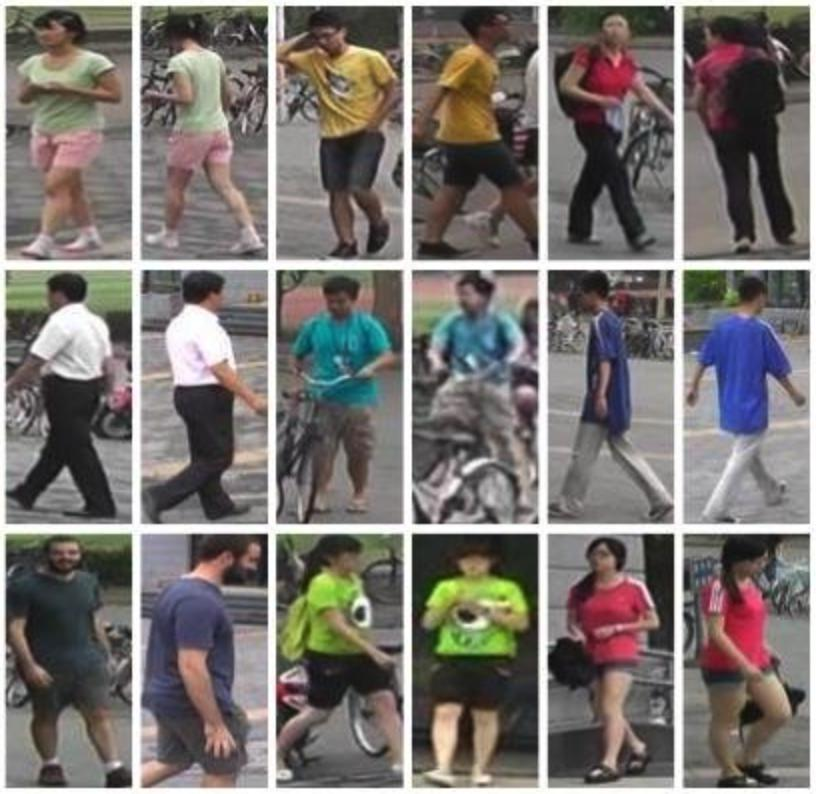
\includegraphics[scale=0.1]
                {fig/intro/motivation/hi_stakes/Market-1501.jpg}};
            \pause
            \node (roadkill) at (cancer.east) {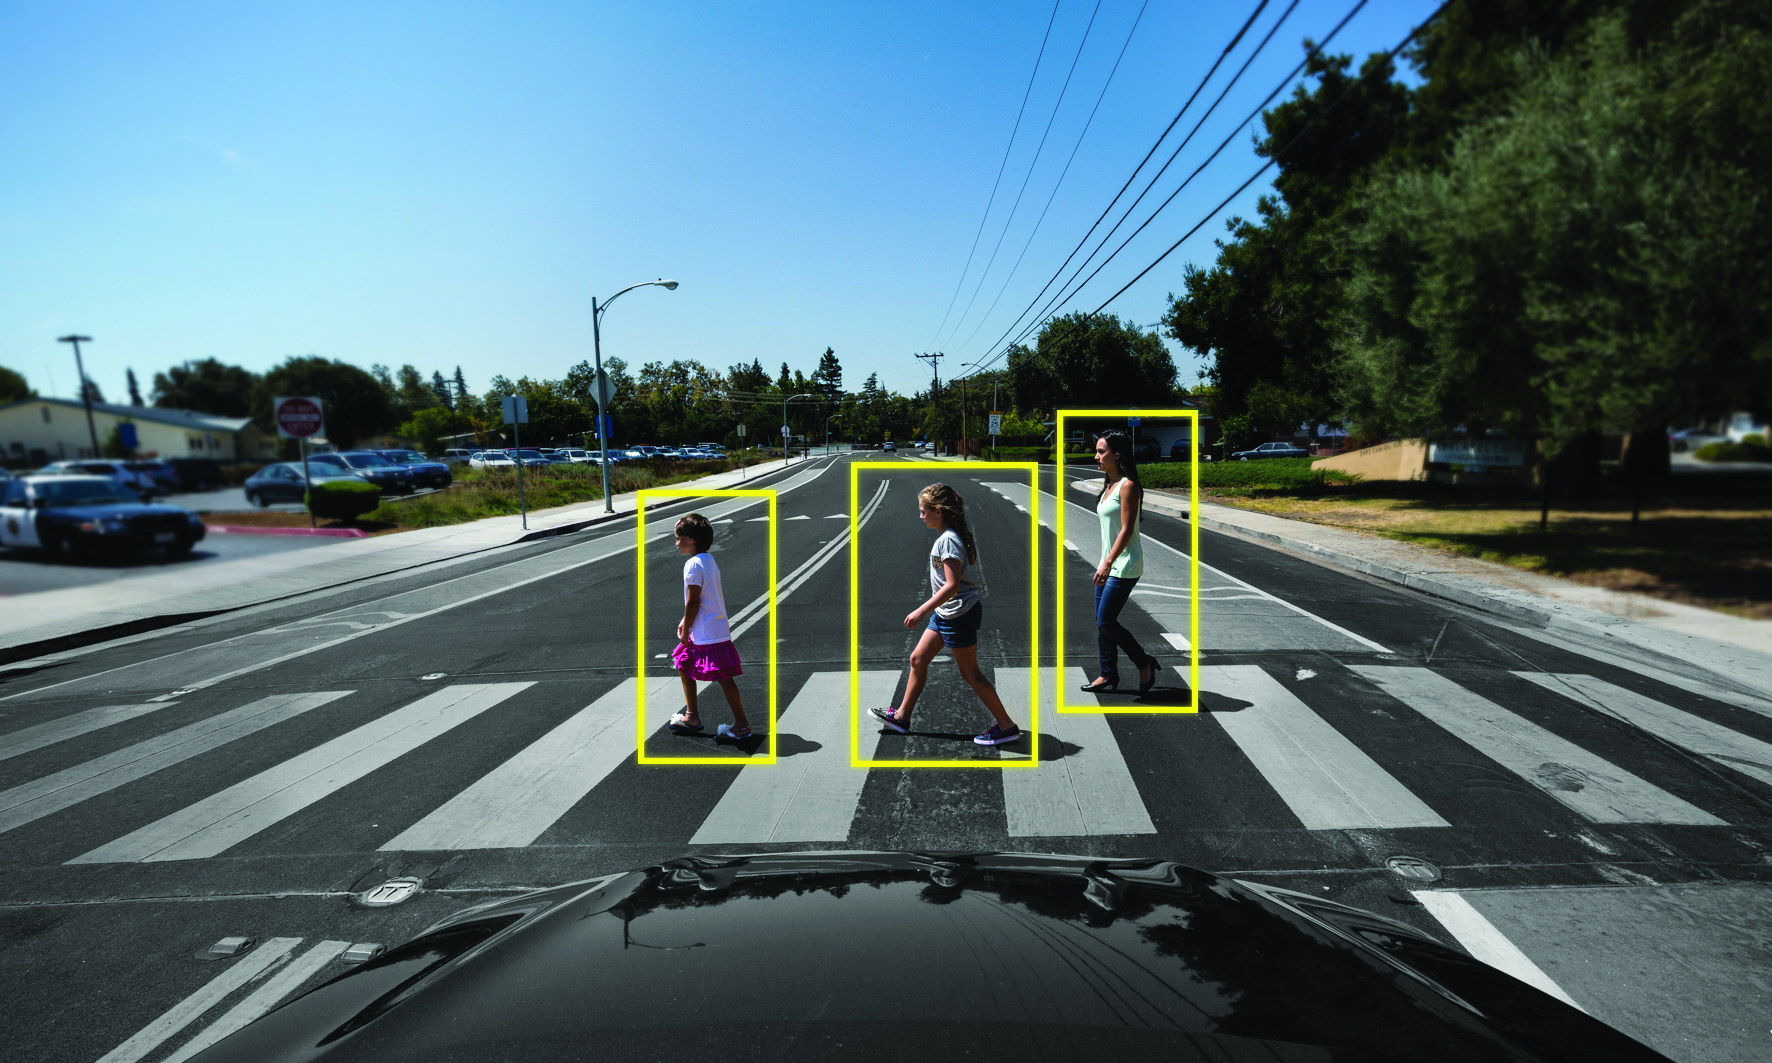
\includegraphics[scale=0.4]
                {fig/intro/motivation/hi_stakes/zebra_crossing.jpg}};
            
        \end{tikzpicture}
    \end{figure}
\end{frame}
 %--------------------------------------------------------------------------------------------------
 \begin{frame}[t]
    \frametitle{Motivation: Straight to the point}
    \begin{columns}
        \column{0.5\textwidth}
        \begin{figure}
            \centering
            \begin{tikzpicture}[font={\scriptsize}]
                \node (cancer) at (current page.north west) 
                    {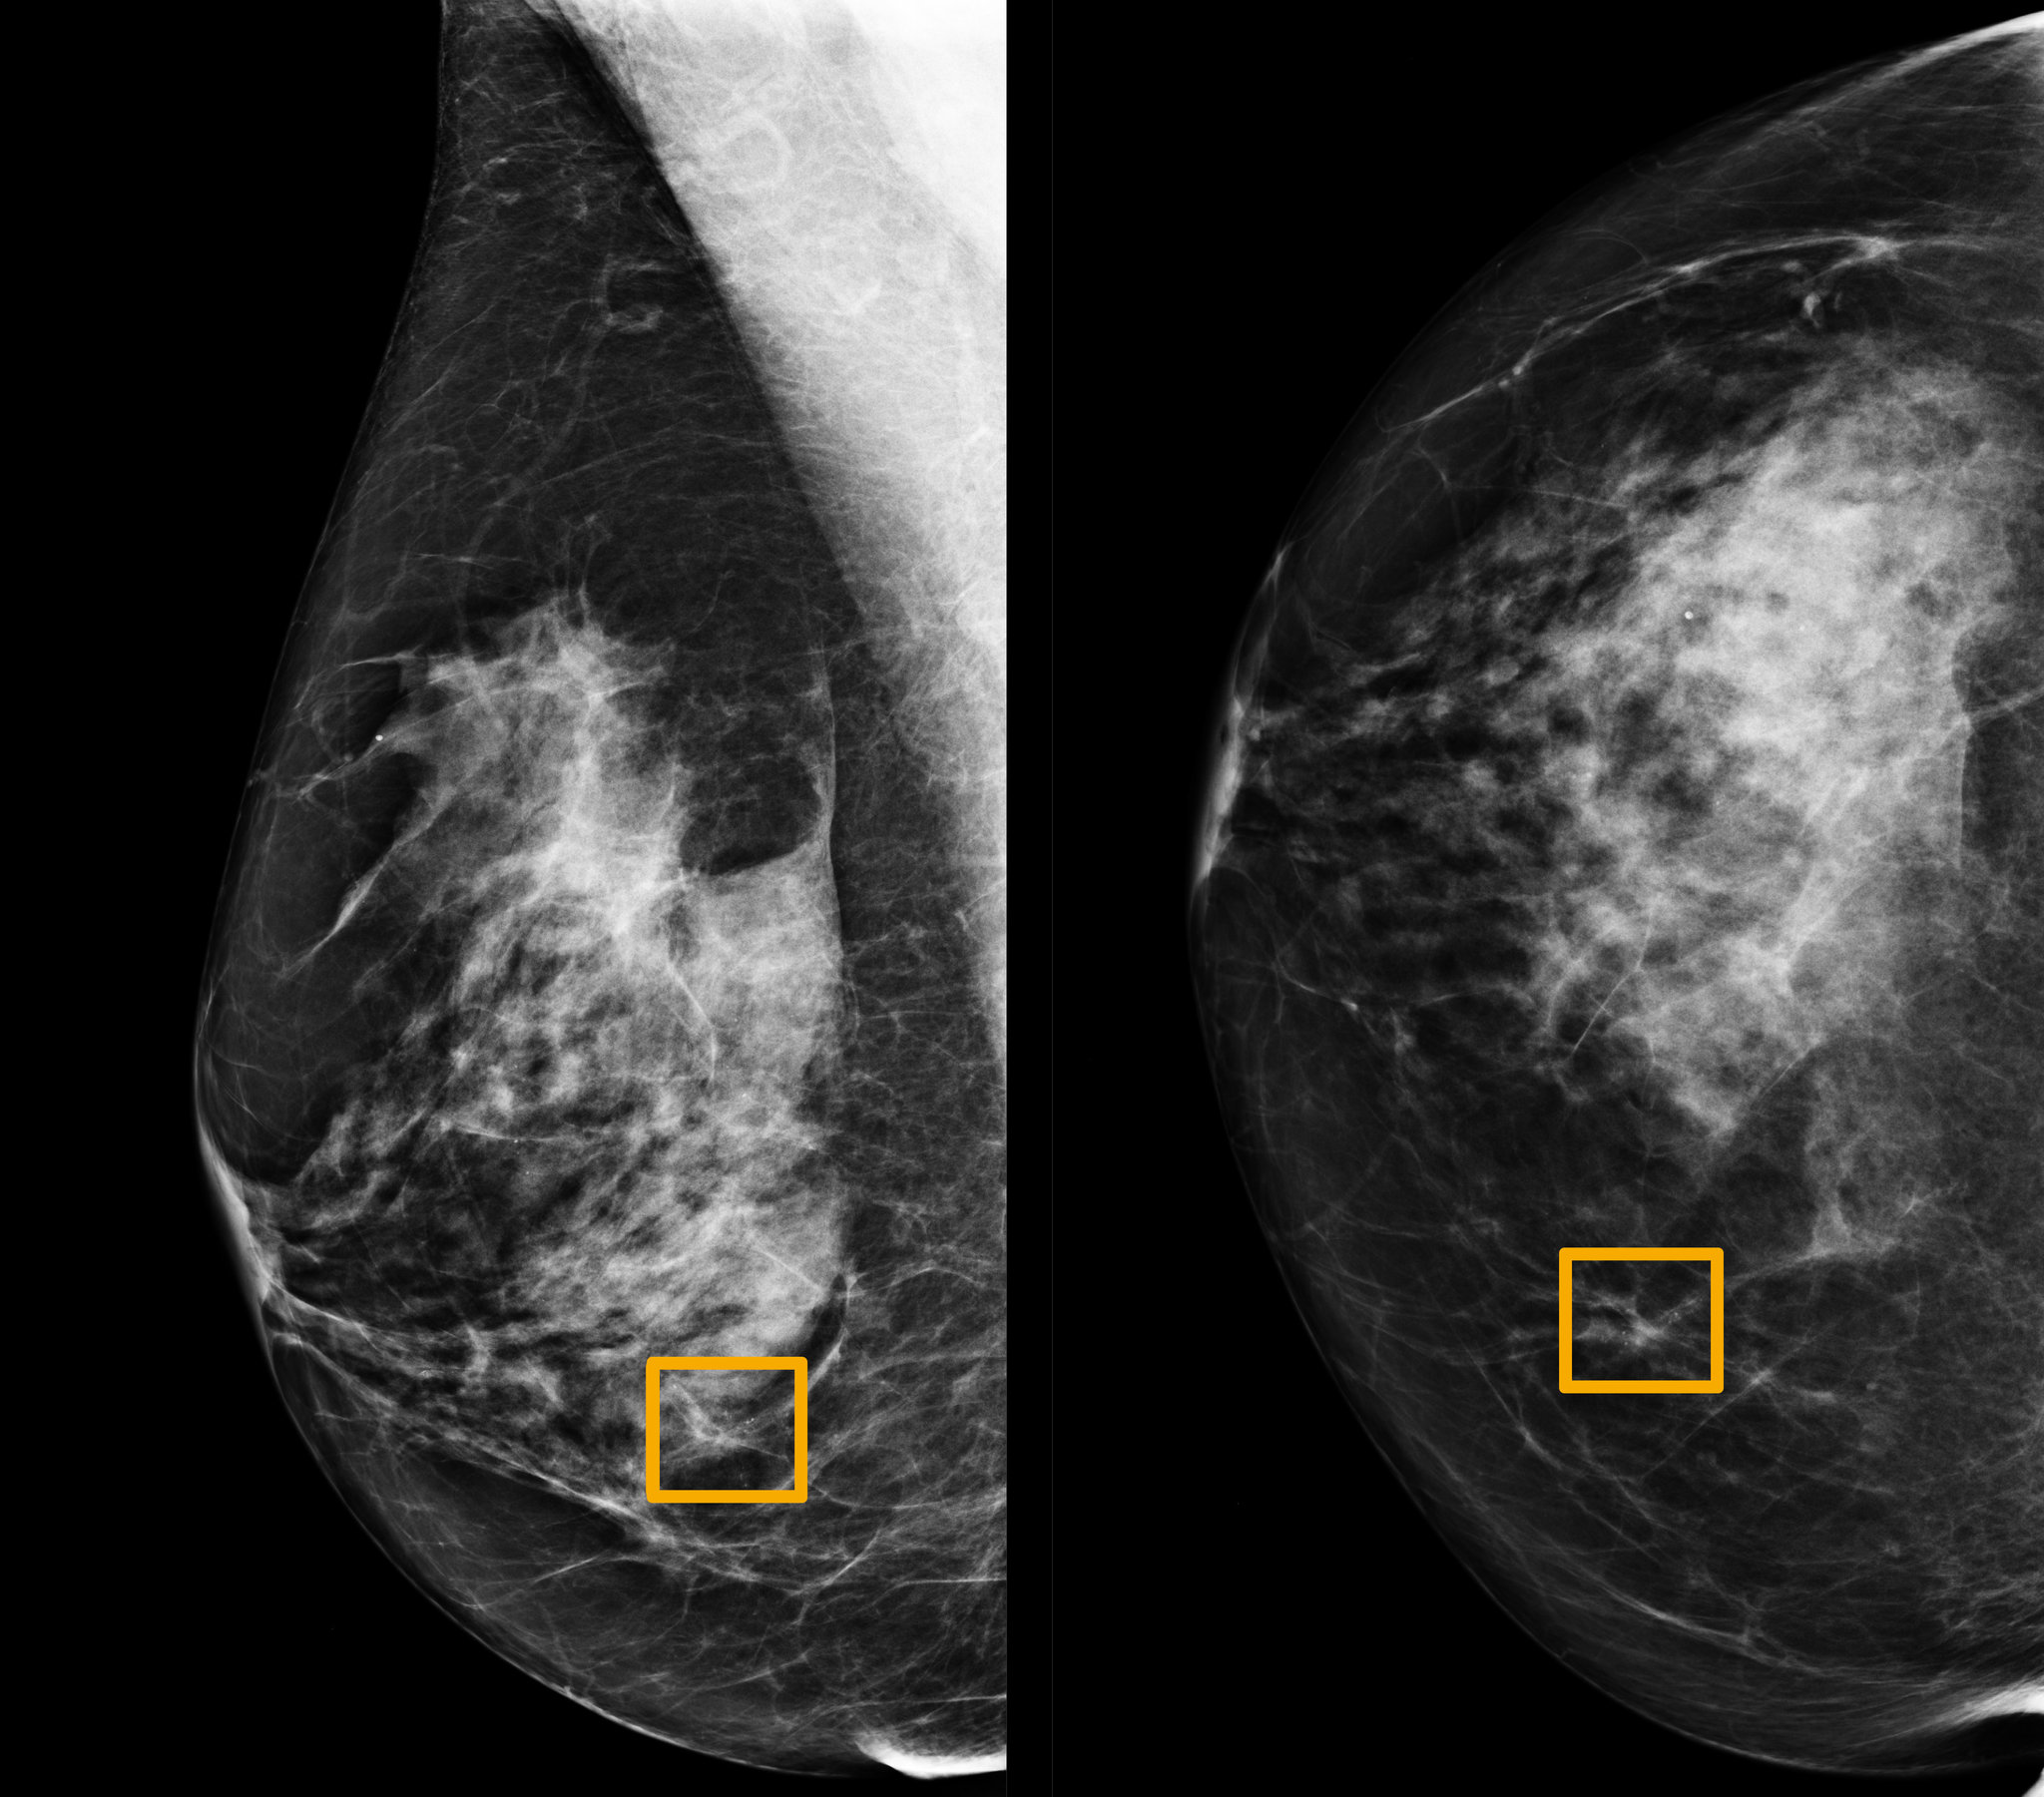
\includegraphics[scale=.05]{fig/intro/motivation/hi_stakes/breast_xray.jpg}};
                \node (roadkill) at (cancer.south) 
                    {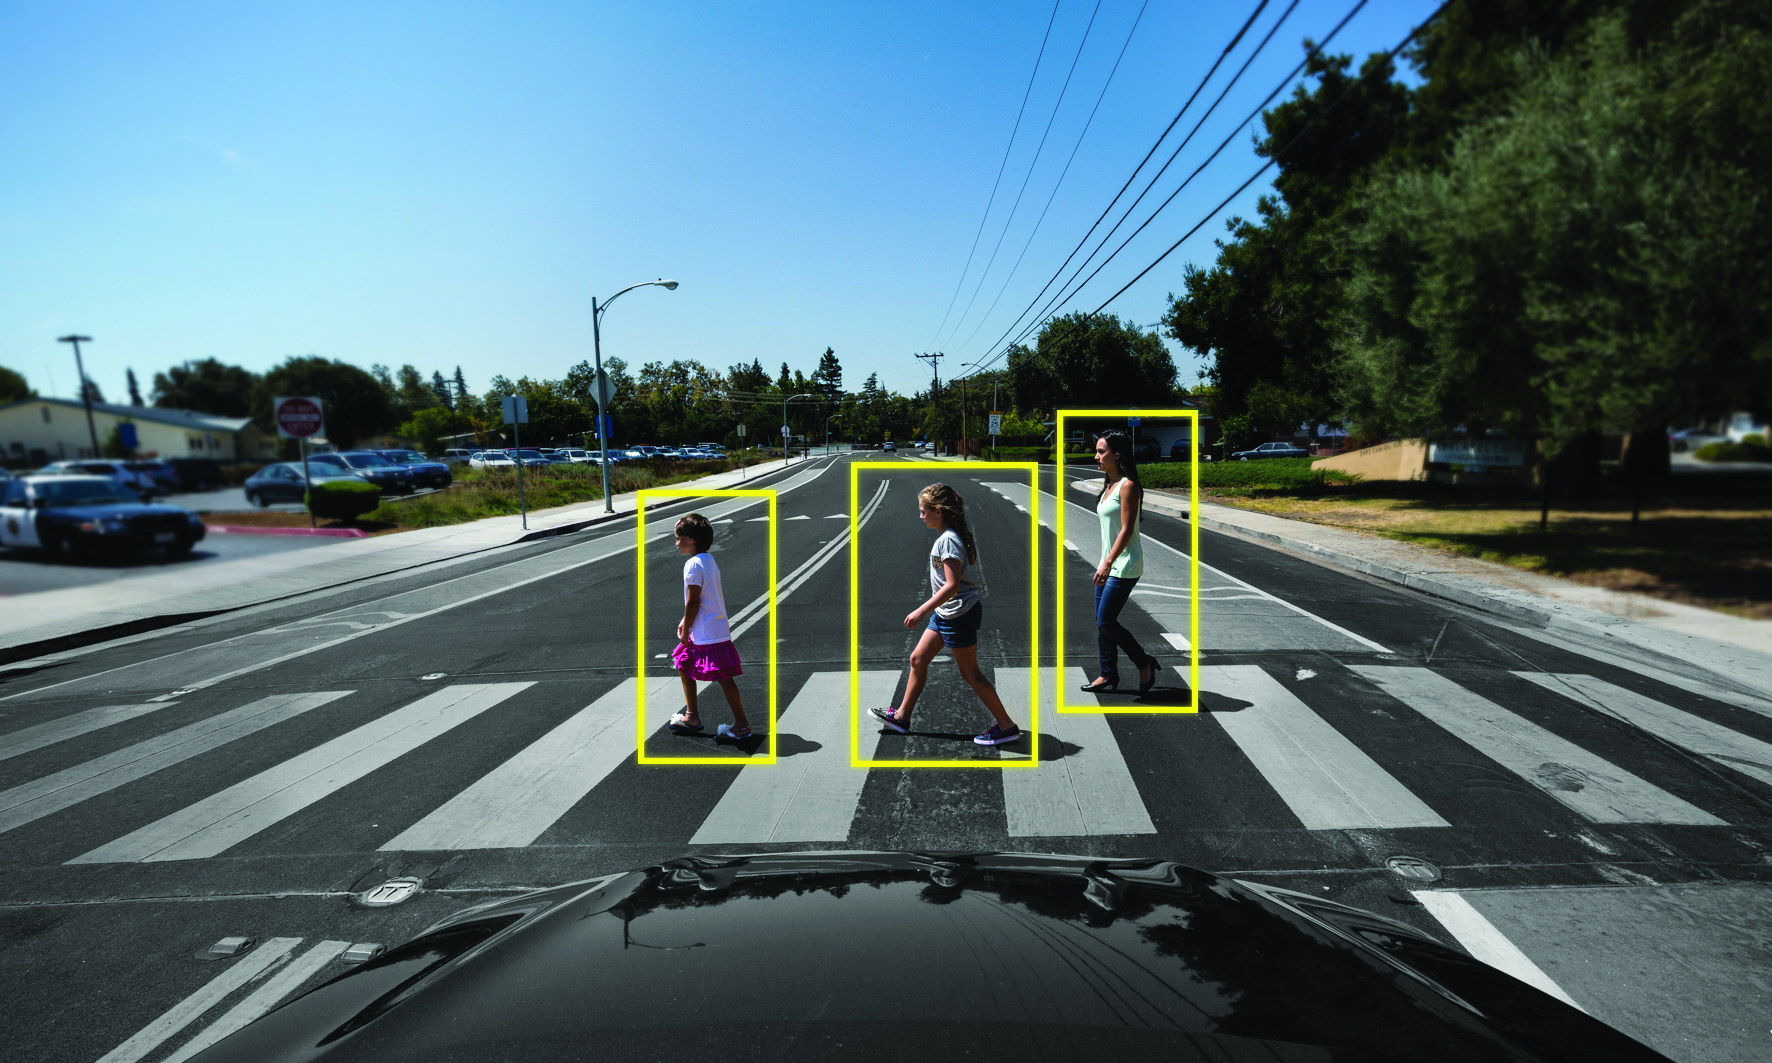
\includegraphics[scale=0.282]{fig/intro/motivation/hi_stakes/zebra_crossing.jpg}};
                \node (reid) at (roadkill.north east) 
                    {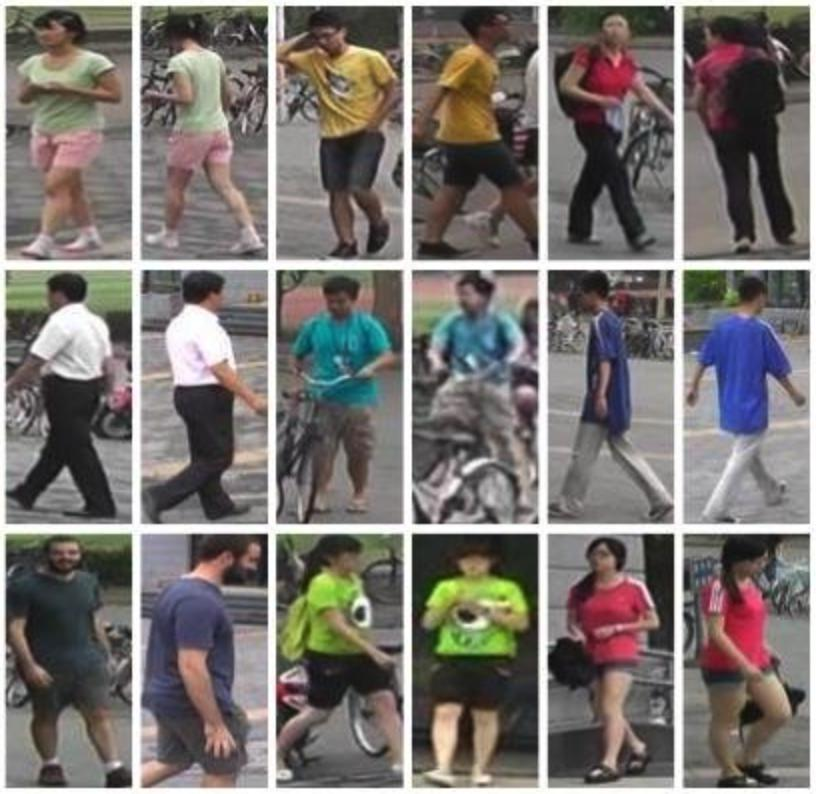
\includegraphics[scale=0.0883]{fig/intro/motivation/hi_stakes/Market-1501.jpg}};                
            \end{tikzpicture}
        \end{figure}
        \column{0.5\textwidth}
            \begin{itemize}
                \item How do we know \textbf{how} safe a system is?\pause
                \item How do we \textbf{know} how a system works?\pause
                \item If a system fails, \textbf{who} is accountable?
            \end{itemize}
        \end{columns}
 \end{frame}
 %--------------------------------------------------------------------------------------------------
\begin{frame}
    \frametitle{}
    \centering
    Let's slow for a bit\\
    and go step by step:   
\end{frame}
%--------------------------------------------------------------------------------------------------
\subsection*{Computation, Computer Vision and AI}
\begin{frame}[t]
    \frametitle{Computation, Computer Vision and AI}
    \cite{mythos_interp}
\end{frame}